\documentclass[12pt]{article}
\usepackage[utf8]{inputenc}
\usepackage{amsmath, amssymb, amsthm}
\newtheorem{question}{Question}
\setlength\parskip{0.5em}
\setlength\parindent{0cm}
\usepackage{hyperref}

\usepackage{tikz}
\usetikzlibrary{shapes, positioning, arrows.meta}

\title{The Four Colour Theorem}
%\author{Mathematics Department}
%\date{\today}

\begin{document}

\maketitle

\section*{Colouring Maps}
The famous Four Colour Theorem has its roots at UCL. In 1852, \textbf{Francis Guthrie}, a mathematics student at the time, noticed that four colours seemed sufficient to colour any map so that no two adjacent regions shared the same colour. He shared this observation with his brother Frederick, who then brought it to the attention of their professor, Augustus De Morgan.

This problem took another 124 years to solve and even today the only known proofs require a computer to verify parts of the argument.

\begin{figure}[h!]
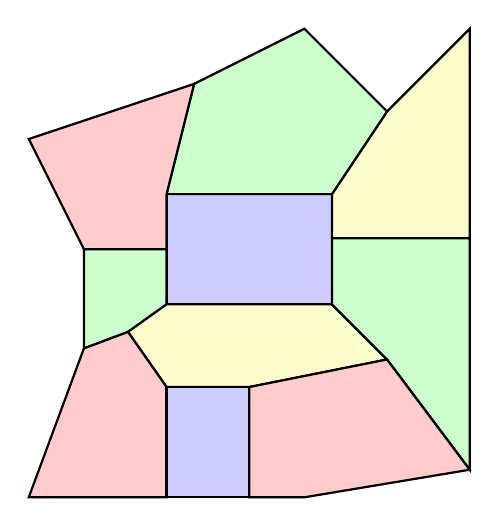
\begin{tikzpicture}[scale=0.7, thick, every node/.style={font=\tiny\bfseries}]
    % Map reproduction with shared coordinates
    \coordinate (P1) at (-1.5, 1);   % GL_NW
    \coordinate (P2) at (1.5, 1);    % GL_NE
    \coordinate (P3) at (1.5, -1);   % GL_SE
    \coordinate (P4) at (-1.5, -1);  % GL_SW
    \coordinate (C_GL_EAST_MID) at (1.5, 0.2); 
    \coordinate (C_GL_WEST_MID) at (-1.5, 0);  
    \coordinate (C_BK_HT) at (-1, 3);
    \coordinate (C_HT_EX) at (2.5, 2.5);
    \coordinate (C_EX_KT) at (4, 0.2);     
    \coordinate (C_KT_SR) at (2.5, -2);
    \coordinate (C_SR_ES) at (1, -2.3);
    \coordinate (C_ES_WS) at (0, -2.5);
    \coordinate (C_WS_HP) at (-1.5, -2.5);
    \coordinate (C_HP_BR) at (-3, -1.8);
    \coordinate (C_BR_BK) at (-3, 0);       
    \coordinate (C_BR_SR_HP) at (-2.2, -1.5); 
    \coordinate (C_HP_WS_B) at (-1.5, -4.5);  
    \coordinate (C_WS_ES_B) at (0, -4.5);     

    % 1. Greater London (GL) - Blue
    \draw[fill=blue!20] (P1) -- (P2) -- (C_GL_EAST_MID) -- (P3) -- (P4) -- (C_GL_WEST_MID) -- cycle;
    \node at (0,0) {};

    % 2. Essex (EX) - Yellow
    \draw[fill=yellow!20] (P2) -- (C_HT_EX) -- (4, 4) -- (C_EX_KT) -- (C_GL_EAST_MID) -- cycle;
    \node at (2.8, 1.8) {};

    % 3. Hertfordshire (HT) - Green
    \draw[fill=green!20] (P1) -- (C_BK_HT) -- (1, 4) -- (C_HT_EX) -- (P2) -- cycle;
    \node at (0.5, 2.5) {};

    % 4. Buckinghamshire (BK) - red
    \draw[fill=red!20] (P1) -- (C_GL_WEST_MID) -- (C_BR_BK) -- (-4, 2) -- (C_BK_HT) -- cycle;
    \node at (-2, 2.3) {};

    % 5. Berkshire (BR) - Green
    \draw[fill=green!20] (C_GL_WEST_MID) -- (P4) -- (C_BR_SR_HP) -- (C_HP_BR) -- (C_BR_BK) -- cycle;
    \node at (-2.5, -0.7) {};

    % 6. Surrey (SR) - Yellow
    \draw[fill=yellow!20] (P4) -- (P3) -- (C_KT_SR) -- (C_SR_ES) -- (C_ES_WS) -- (C_WS_HP) -- (C_BR_SR_HP) -- cycle;
    \node at (0.2, -1.8) {};

    % 7. Kent (KT) - Green
    \draw[fill=green!20] (P3) -- (C_GL_EAST_MID) -- (C_EX_KT) -- (4, -4) -- (C_KT_SR) -- cycle;
    \node at (3, -1) {};

    % 8. Hampshire (HP) - red
    \draw[fill=red!20] (C_BR_SR_HP) -- (C_WS_HP) -- (C_HP_WS_B) -- (-4, -4.5) -- (C_HP_BR) -- cycle;
    \node at (-2.8, -2.5) {};

    % 9. West Sussex (WS) - Blue
    \draw[fill=blue!20] (C_WS_HP) -- (C_ES_WS) -- (C_WS_ES_B) -- (C_HP_WS_B) -- cycle;
    \node at (-0.7, -3.5) {};

    % 10. East Sussex (ES) - red
    \draw[fill=red!20] (C_ES_WS) -- (C_SR_ES) -- (C_KT_SR) -- (4, -4) -- (1, -4.5) -- (C_WS_ES_B) -- cycle;
    \node at (1.8, -3.5) {};

\end{tikzpicture}
\hskip 2cm
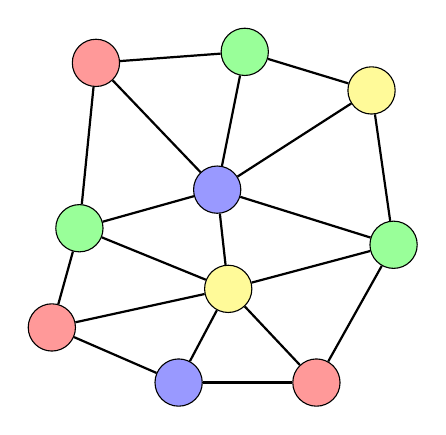
\begin{tikzpicture}[scale=0.7, every node/.style={circle, draw, minimum size=0.6cm, font=\tiny\bfseries}]
    % Dual Graph
    \node[fill=blue!40]   (V_GL) at (0,0){};
    \node[fill=yellow!40] (V_EX) at (2.8, 1.8) {};
    \node[fill=green!40]  (V_HT) at (0.5, 2.5) {};
    \node[fill=red!40] (V_BK) at (-2.2, 2.3) {};
    \node[fill=green!40]  (V_BR) at (-2.5, -0.7) {};
    \node[fill=yellow!40] (V_SR) at (0.2, -1.8) {};
    \node[fill=green!40]  (V_KT) at (3.2, -1) {};
    \node[fill=red!40] (V_HP) at (-3, -2.5) {};
    \node[fill=blue!40]   (V_WS) at (-0.7, -3.5) {};
    \node[fill=red!40] (V_ES) at (1.8, -3.5) {};
    
    % Adjacencies (Edges) - Solid Lines
    \draw[thick] (V_GL) -- (V_EX); \draw[thick] (V_GL) -- (V_HT); \draw[thick] (V_GL) -- (V_BK);
    \draw[thick] (V_GL) -- (V_BR); \draw[thick] (V_GL) -- (V_SR); \draw[thick] (V_GL) -- (V_KT);
    
    \draw[thick] (V_HT) -- (V_BK); \draw[thick] (V_HT) -- (V_EX);
    \draw[thick] (V_BK) -- (V_BR); \draw[thick] (V_EX) -- (V_KT);
    
    \draw[thick] (V_BR) -- (V_SR); \draw[thick] (V_BR) -- (V_HP);
    \draw[thick] (V_SR) -- (V_KT); \draw[thick] (V_SR) -- (V_ES); \draw[thick] (V_SR) -- (V_WS); \draw[thick] (V_SR) -- (V_HP);
    
    \draw[thick] (V_KT) -- (V_ES);
    \draw[thick] (V_HP) -- (V_WS); \draw[thick] (V_WS) -- (V_ES);
    
\end{tikzpicture}
\caption{A 4-coloured map and its 4-coloured dual graph}\label{dual}
\end{figure}
Rather than thinking about map colouring directly, we can look at the \emph{dual} problem (see Figure \ref{dual}). Each region in the map becomes a \emph{vertex} and  we draw an \emph{edge} between two vertices if their corresponding regions share a border. A colouring of the map is then equivalent to a ``vertex colouring'' of this dual graph, where no two adjacent vertices have the same colour.

This dual object is called a \emph{planar graph}. The key property of a planar graph is that it can be drawn on a piece of paper so that no two edges cross (remember edges are the straight lines and vertices are the dots we colour).


If we look again at the example in Figure \ref{dual} it isn't hard to see that we can actually colour it with three colours, as shown in Figure \ref{3col}. 
\begin{question}[Warm-up]
Can you find an example of a planar graph that requires four colours to colour it properly (no two adjacent vertices have the same colour)? 
\end{question}
\begin{figure}
\begin{center}
    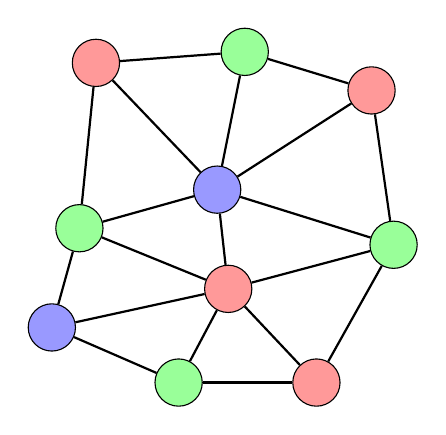
\begin{tikzpicture}[scale=0.7, every node/.style={circle, draw, minimum size=0.6cm, font=\tiny\bfseries}]
    % Dual Graph
    \node[fill=blue!40]   (V_GL) at (0,0) {};
    \node[fill=red!40] (V_EX) at (2.8, 1.8) {};
    \node[fill=green!40]  (V_HT) at (0.5, 2.5) {};
    \node[fill=red!40] (V_BK) at (-2.2, 2.3) {};
    \node[fill=green!40]  (V_BR) at (-2.5, -0.7) {};
    \node[fill=red!40] (V_SR) at (0.2, -1.8) {};
    \node[fill=green!40]  (V_KT) at (3.2, -1) {};
    \node[fill=blue!40] (V_HP) at (-3, -2.5) {};
    \node[fill=green!40]   (V_WS) at (-0.7, -3.5) {};
    \node[fill=red!40] (V_ES) at (1.8, -3.5) {};
    
    % Adjacencies (Edges) - Solid Lines
    \draw[thick] (V_GL) -- (V_EX); \draw[thick] (V_GL) -- (V_HT); \draw[thick] (V_GL) -- (V_BK);
    \draw[thick] (V_GL) -- (V_BR); \draw[thick] (V_GL) -- (V_SR); \draw[thick] (V_GL) -- (V_KT);
    
    \draw[thick] (V_HT) -- (V_BK); \draw[thick] (V_HT) -- (V_EX);
    \draw[thick] (V_BK) -- (V_BR); \draw[thick] (V_EX) -- (V_KT);
    
    \draw[thick] (V_BR) -- (V_SR); \draw[thick] (V_BR) -- (V_HP);
    \draw[thick] (V_SR) -- (V_KT); \draw[thick] (V_SR) -- (V_ES); \draw[thick] (V_SR) -- (V_WS); \draw[thick] (V_SR) -- (V_HP);
    
    \draw[thick] (V_KT) -- (V_ES);
    \draw[thick] (V_HP) -- (V_WS); \draw[thick] (V_WS) -- (V_ES);
    
\end{tikzpicture}
\end{center}
\caption{A 3-colouring of the dual graph}\label{3col}
\end{figure}

\begin{figure}[h]
\begin{center}
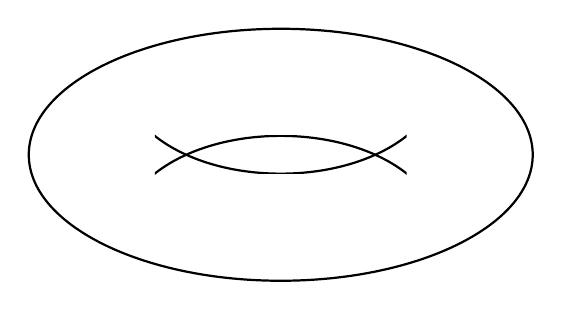
\begin{tikzpicture}[scale=0.8]
    % Torus schematic (isometric view)
    \draw[thick] (0,0) ellipse (4cm and 2cm);
    \begin{scope}
        \clip (-2,-0.3) rectangle (2,1);
        \draw[thick] (0,1.2) ellipse (2.5cm and 1.5cm);
    \end{scope}
    \begin{scope}
        \clip (-2,0.3) rectangle (2,-1);
        \draw[thick] (0,-1.2) ellipse (2.5cm and 1.5cm);
    \end{scope}
\end{tikzpicture}
\end{center}\caption{A doughnut (otherwise known as a torus)}\label{torus}
\end{figure}

It turns out that the question of how many colours are needed to colour graphs drawn on a doughnut (or \emph{torus} as mathematicians call it) is easier to answer than the planar case. To start with let us try to find the largest \emph{clique} that can be drawn on a torus. (A \emph{clique} is a graph in which every vertex is connected to every other vertex.)
\begin{question}
What is the largest clique that can be drawn on a torus?
\end{question}
Drawing a graph on a torus can be hard to visualize, but there is a nice trick we can use to help us. We can draw the graph on a piece of paper and then roll it up into a cylinder, identifying the left and right edges. Then we can can roll the cylinder up into a torus, identifying the top and bottom circles of the cylinder. (In practice doing this by hand with a piece of paper is not easy, so here is an online tool to help you explore this problem \url{https://www.homepages.ucl.ac.uk/~ucahjmt/doughnut/} and find the answer.)



\section*{Why does 7 suffice?}
The key idea is the following: if every graph that can be drawn on a torus contains a vertex that belongs to at most 6 edges then we can colour the graph with 7 colours "by induction". [More formally: we can easily colour any graph with at most 7 vertices using 7 colours -- simply give each vertex a different colour. Now suppose we have a graph with $n>7$ vertices. If we can find a vertex $v$ that belongs to at most 6 edges, we can remove it from the graph, colour the remaining $n-1$ vertices with 7 colours (by our inductive hypothesis), and then colour $v$ with one of the colours that is not used by any of its neighbours (since $v$ has at most 6 neighbour there is always a colour available).]

So how do we show that any graph that can be drawn on the torus contains a vertex that belongs to at most 6 edges?

There is a magical formula (called the Euler characteristic) that tells us how the number of vertices ($V$), edges ($E$), and faces ($F$) of a graph drawn on a surface are related. 

For a torus the formula says that: 
\[
V =  E - F.\]
Now any face of a graph contains at least 3 edges, and each edge belongs to exactly 2 faces so this tells us that $2E \ge 3F$, so 
\[
6V = 6E - 6F \le 6E - 4E = 2E.
\]
This tells us that the average number of edges a verex belongs to is 6, which means that there must be at least one vertex that belongs to at most 6 edges!
\end{document}

\subsection*{Colouring Complete Graphs and Cycles}
The minimum number of colours needed to colour a graph is called its \textbf{chromatic number}, denoted $\chi(G)$.

As a warm-up question can you work out how many colours we need to colour the following graphs?


\begin{enumerate}
    \item \textbf{Complete Graphs ($K_n$)}: Since every vertex is connected to every other vertex, every vertex must have a unique colour. Thus, $\chi(K_n) = n$.
\end{enumerate}

\begin{center}
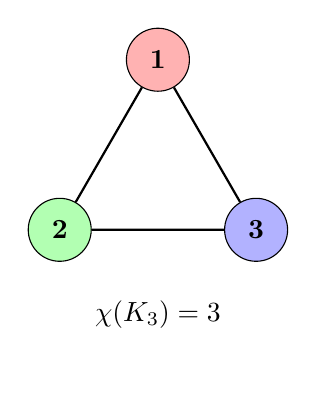
\begin{tikzpicture}[scale=1.2, every node/.style={circle, draw, minimum size=0.8cm, font=\bfseries}]
    \node[fill=red!30] (A) at (90:1.2) {1};
    \node[fill=green!30] (B) at (210:1.2) {2};
    \node[fill=blue!30] (C) at (330:1.2) {3};
    \draw[thick] (A) -- (B) -- (C) -- (A);
    \node[draw=none, fill=none] at (0,-1.5) {$\chi(K_3) = 3$};
\end{tikzpicture}
\end{center}

\begin{enumerate}
    \setcounter{enumi}{1}
    \item \textbf{Cycles ($C_n$)}: A cycle consists of vertices connected in a single loop. 
    \begin{itemize}
        \item If $n$ is even, we can alternate between 2 colours: $\chi(C_{\text{even}}) = 2$.
        \item If $n$ is odd, the last vertex will always conflict with the first if we only have 2 colours: $\chi(C_{\text{odd}}) = 3$.
    \end{itemize}
\end{enumerate}

\begin{center}
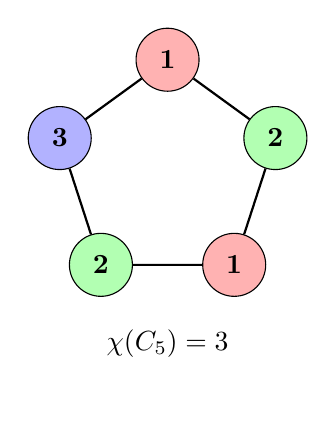
\begin{tikzpicture}[scale=1.2, every node/.style={circle, draw, minimum size=0.8cm, font=\bfseries}]
    \node[fill=red!30] (1) at (90:1.2) {1};
    \node[fill=green!30] (2) at (18:1.2) {2};
    \node[fill=red!30] (3) at (306:1.2) {1};
    \node[fill=green!30] (4) at (234:1.2) {2};
    \node[fill=blue!30] (5) at (162:1.2) {3};
    \draw[thick] (1) -- (2) -- (3) -- (4) -- (5) -- (1);
    \node[draw=none, fill=none] at (0,-1.8) {$\chi(C_5) = 3$};
\end{tikzpicture}
\end{center}


\section*{Question 1: Planarity and Complete Graphs}
A complete graph $K_n$ is a graph where every vertex is connected to every other vertex by a unique edge.

\begin{enumerate}
    \item Show that for any simple planar graph, $E \le 3V - 6$. (Hint: Every face must have at least 3 edges).
    \item Use this inequality to prove that $K_5$ is not planar, but $K_4$ is.
    \item Below is an illustration of $K_4$ drawn without any edges crossing.
\end{enumerate}

\begin{center}
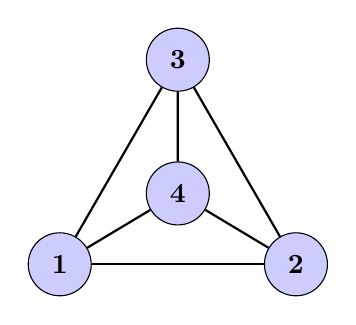
\begin{tikzpicture}[scale=1.5, every node/.style={circle, fill=blue!20, draw, minimum size=0.8cm, font=\bfseries}]
    % Define vertices of K4
    \node (A) at (0, 0) {1};
    \node (B) at (2, 0) {2};
    \node (C) at (1, 1.732) {3};
    \node (D) at (1, 0.6) {4};

    % Draw edges for planar K4
    \draw[thick] (A) -- (B);
    \draw[thick] (B) -- (C);
    \draw[thick] (C) -- (A);
    \draw[thick] (A) -- (D);
    \draw[thick] (B) -- (D);
    \draw[thick] (C) -- (D);
\end{tikzpicture}
\end{center}

\section*{Question 2: Graphs on a Torus}
Now imagine we are drawing our graph on a torus (a surface with one hole).

\begin{enumerate}
    \item Using Euler's formula for a torus ($V - E + F = 0$), derive the equivalent inequality for the number of edges: $E \le 3V$.
    \item A complete graph $K_n$ has $E = \frac{n(n-1)}{2}$ edges. Calculate the maximum value of $n$ such that $K_n$ can be embedded on a torus without any edges crossing.
    \item Why does this imply that while maps on a plane require 4 colours, maps on a torus can require up to 7?
\end{enumerate}
